\documentclass{subfiles}

\begin{document}

	

\section{Introduction}


\par To briefly sum up the previous sections, FW LiDAR data (Section \ref{AcquireData}) are laser scanning data particularly useful in Forestry, but the huge amount of information recorded make handling of the data difficult. The open source software DASOS (Section \ref{DASOS}) was developed along with this thesis to ease the usage of the data. DASOS voxelises (Section \ref{Voxelisation}) the data before interpretation and this approach is fundamentally different from the related and state-of-art software packages. The output of the voxelisation is a 3D discrete density Volume. 


\par This chapter explains the concepts of reconstructing the surface of the scanned area from the 3D voxelised FW LiDAR. At first, volumetric rendering approaches are briefly described at Section\ref{sec:RenderingApproaches}. Section \ref{sec:AlgebracObjects} gives a mathematical definition to the voxelised data, while Section \ref{sec:SurfaceReconstruction} explains the actual algorithm of generating a surface from the voxelised FW LiDAR data. By the end the results are given in Section \ref{sec:MCResults}. 


\section{Rendering Approaches of Volumetric Data}\label{sec:RenderingApproaches}
\par Even though the concept of visualising 3D discrete density volumes (Volumetric Visualisations) is new in forestry and remote sensing, it has been widely research in medical imaging and visual effects. There are two approaches of visualising volumetric data.

\par The first approach is direct rendering, which repeatedly generates 2D images according to the view point (the camera). It is like "taking photos" from a camera and putting them in a sequence to produce an interactive video. An example of direct rendering approach is ray-tracing. Ray-tracing generates images by "taking photos"; rays are casted from the view point passing through each pixel and intensity values are assigned to the pixels according to the nearest intersections \cite{Hanrahan1983}. Ray-tracing can be time expensive depending on the complexity of the scene. Most of the direct rendering literature focuses on parallellising the ray-casting process. By introducing parallelisation, real time rendering of small volumetric data ($256^3$) was achieved by Pfister et al in 1999 \cite{Pfister1999} and after the release of the CUDA hardware (which is a parallel computing platform on recent nvidia graphics cards), in 2009 Crassin et al achieved real-time rendering of billions of voxels \cite{Crassin2009}. 
	
\par Even though it is possible to implement real-time interactive environments using direct rendering of the big voxel data, volumetric visualisations of FW LiDAR data is a new concept in remote sensing and for simplicity, this thesis experiments surface reconstruction (the second approach). Surface reconstruction refers to the extraction of a polygonal mesh, which is a set of primitives like triangles, from the volumetric data. Constructing a surface may take several minutes, but real time visualisations of polygonal meshes are supported by free animation packages (like Blender and Meshlab) and it work on commodity hardware. This is achieved with rasterisation, which is a method that maps the primitives to pixels, it is widely used in computer games and it is significantly faster than ray-tracing. Furthermore, interactive operations (e.g. measuring the distance between two trees) are trivial calculations on primitives/polygonal meshes and they are easy to implement. 



\section{Algebraic Definition of the Volume}\label{sec:AlgebracObjects}

In computer graphics, polygonal meshes are a set of primitives usually triangles, but some objects are defined differently, for example using a function. Those objects are called either implicit or algebraic. Implicit representation of objects allows a mathematical definition to the 3D discrete density volume generated from the FW LiDAR data (Section \ref{Voxelisation}). 

\par Algebraic objects were introduced by Blinn in 1982 \cite{Blinn1982} to enable the definition of complex objects without saving a large amount of primitives. Each one is defined by a function $ \mathit{f(X)} $ and the iso-surface value $\alpha$. The iso-surface value (iso-level) defines the boundaries of the object; for an object $ [f(x),a]$ every n-dimensional point $ \mathit{X} $  that lies on the surface of the object satisfies the condition $ \mathit{f(X)=\alpha }  $. To be more accurate, the following rules apply according to Pasko et al \cite{Pasko1994}: 
\begin{itemize}
	\item $	\mathrm{f(X) = \alpha }$ , when $X$ lies on the surface of the algebraic object
	\item $	\mathrm{f(X) > \alpha }$ , when $X$ lies inside the algebraic object and
	\item $	\mathrm{f(X) < \alpha }$ , when $X$ lies outside the algebraic object	 
\end{itemize}

\par Regarding the algebraic representation of the 3D voxelised FW LiDAR data, X is a three dimensional point $\mathit{(x, y, z) }$ representing the longitude, latitude and height respectively and ${f(X)}$ is a function that takes  $\mathit{X}$ as input and returns the accumulated intensity value of the voxel that  $\mathit{X}$ lies inside. Also, the iso-surface value $\mathit{\alpha }$ is a user defined parameter and it is noise dependant (Please look at figure \ref{fig:SwitchingVisParameters} to understand how the iso-surface value / iso-level affects the output of the surface reconstruction of the voxelised FW LiDAR data). 




\section {Surface Reconstruction with the Marching Cubes Algorithm}\label{sec:SurfaceReconstruction}

\par Even though numerical implicitisation is beneficial in reducing storage memory and for multiple resolution renderings of the same object, visualising implicit objects is not straight forward, since they contain no discrete values. This problem can either be address either by direct rendering or surface reconstruction (Section \ref{sec:RenderingApproaches}). 

\par The Marching Cubes algorithm is an algorithm that polygonises implicit objects using a look up table. Let’s assume that $f(X)$ defines an implicit object. At first the space is divided into cubes. Each cube is defined by eight corner points, which lie either inside or outside the object. By enumerating all the possible cases and linearly interpolating the intersections along the edges, the surface of the implicit object is constructed \cite{Lorensen1987}. 

\par According to Lorensen and Cline \cite{Lorensen1987}, the normal\footnote{The normal in geometry is a vector that is perpendicular to the surface of a polygonal object. In graphics, each vertex is is associated with a normal to allow visualisations of smooth objects. The normal is further important for estimating light illumination during rendering.} of each vertex is calculated by measuring the local gradient change. Even though this gives an accurate result on smooth object (e.g. a spherical object defined by the equation of a sphere), the voxelised FW LiDAR data contain high gradient changes. Therefore, this approach results into normals pointing into inconsistent directions and when rendered the surface appears rough. For that reason, in DASOS the normal of each vertex is derived by the average normal of its adjacent triangles. 

\par Additionally it worth highlighting that the sampling of the Marching cubes is independent from the sampling of the 3D density volume. But consistency between the two is required (Figure \ref{fig:MCSampling}). Let’s assume the discrete volume has (n * m * k) voxels. The volume can be sampled into cubes at any rate but to reduce artifacts a ((n+1) *(m+1) * (k+1)) dimensional sampling is suggested. Please note that every point that lies outside the volume is considered to be below the boundary threshold and set to a value lower than the isosurface value. An example of the corresponding sampling in 2D is shown on Figure 1, where the black grid represents a 2D density table and the blue grid represents the sampling used in during polygonisation.

\par The following Figura \ref{fig:SamplingArtifacts} shows the effects of oversampling during polygonisation. The right image was oversampled and the second one was sampled as explained above.

    %% Sampling
    \begin{figure} [h!]
    	\begin{subfigure}[t]{.49\textwidth}
    		
    		\centering
    		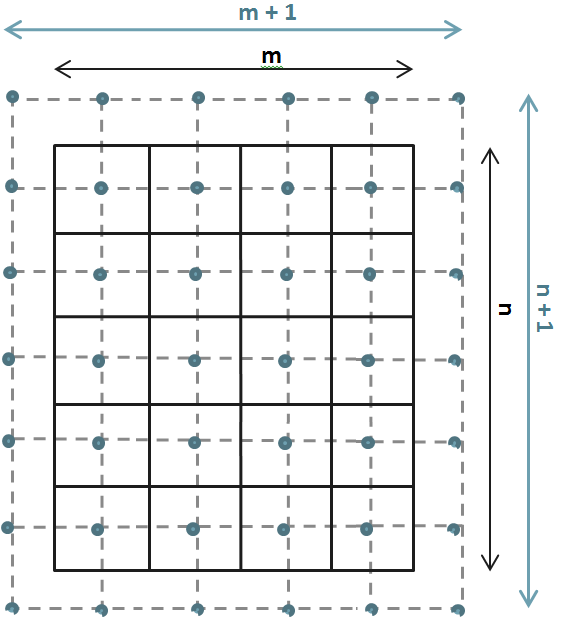
\includegraphics[width=.9\textwidth]{img/Sampling}
    		\caption{Suggested Sampling}
    		\label{fig:ExpectedSampling}
    	\end{subfigure} \hfill
    	\begin{subfigure}[t]{.49\textwidth}
    		\centering
    		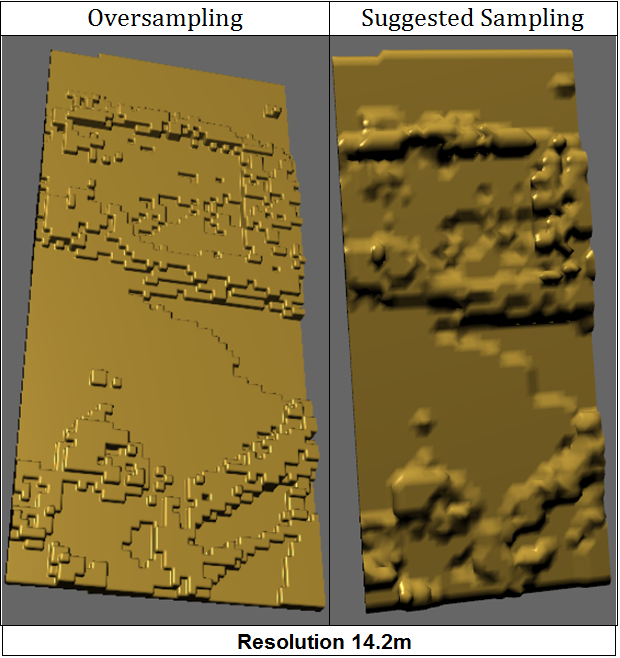
\includegraphics[width=.9\textwidth]{img/OversamplingVsSuggestedSampling}
    		\caption{Artifacts of Oversampling} 
    		\label{fig:SamplingArtifacts}
    	\end{subfigure} \hfill
    	\caption[Marching Cubes Sampling]{The suggested sampling during polygonisation using the Marching Cubes Algorithm}
    	\label{fig:MCSampling}
    \end{figure}


\section{Results}\label{sec:MCResults}

 
 selecting region of interest \&
 

 \begin{figure} [h!]
 	\centering
 	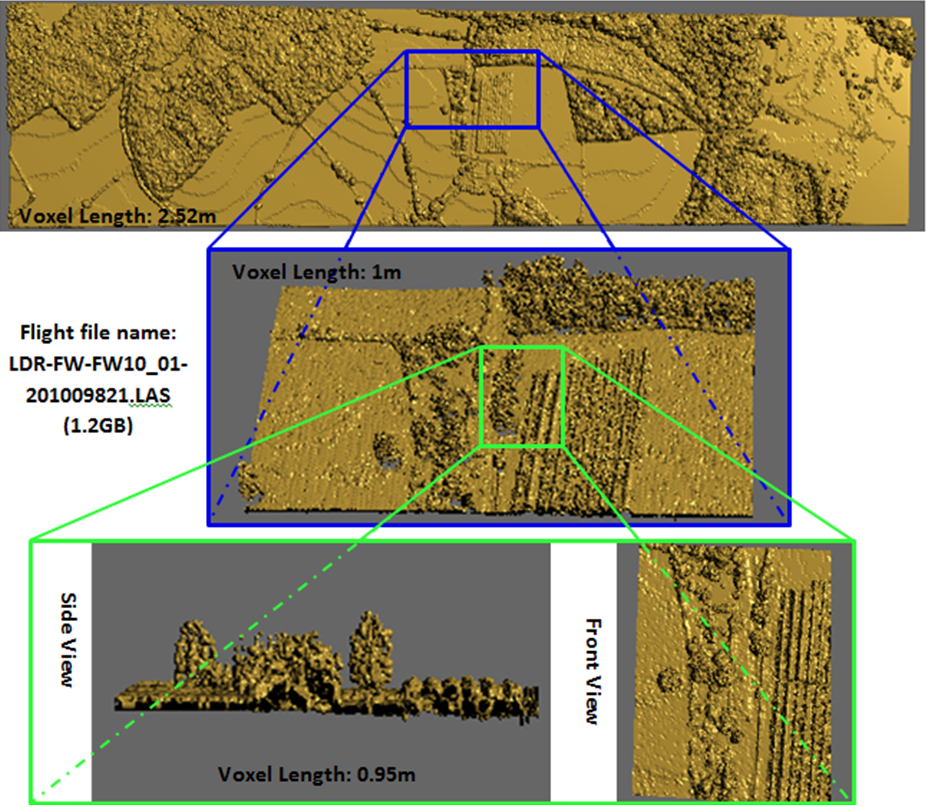
\includegraphics[width=.8\textwidth]{img/SelectingRegionOfInterest}
 	\caption[Selecting Region of Interest]{Selecting Region of Interest}
 	\label{fig:SelectingRegionOfInterest}
 \end{figure}
 
 
  \begin{figure} [h!]
  	\centering
  	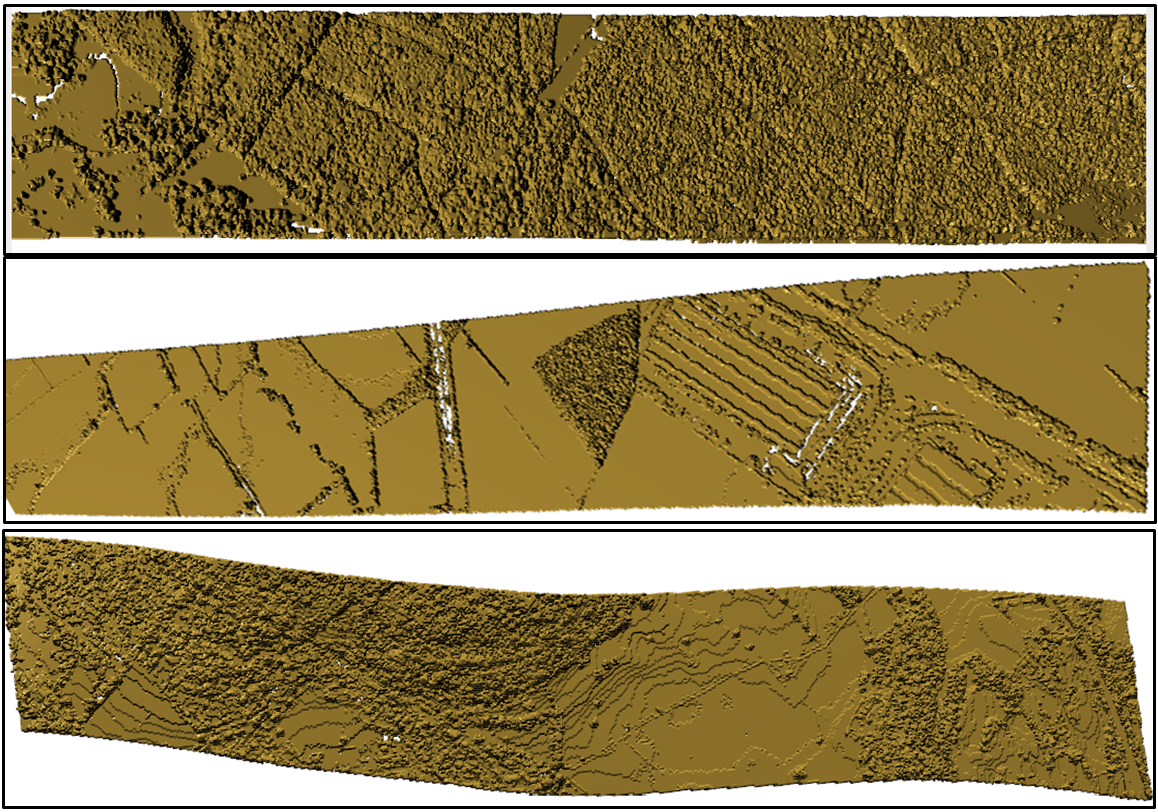
\includegraphics[width=.8\textwidth]{img/VariousFlightlines}
  	\caption[Various Flightlines Visualisation]{Polygonising NERC-ARF FW LiDAR data captured at different areas (New Forest, Milton Keynes and Eaves Wood)}
  	\label{fig:VariousFlightlines}
  \end{figure}
  

  
  \begin{figure} [h!]
  	\centering
  	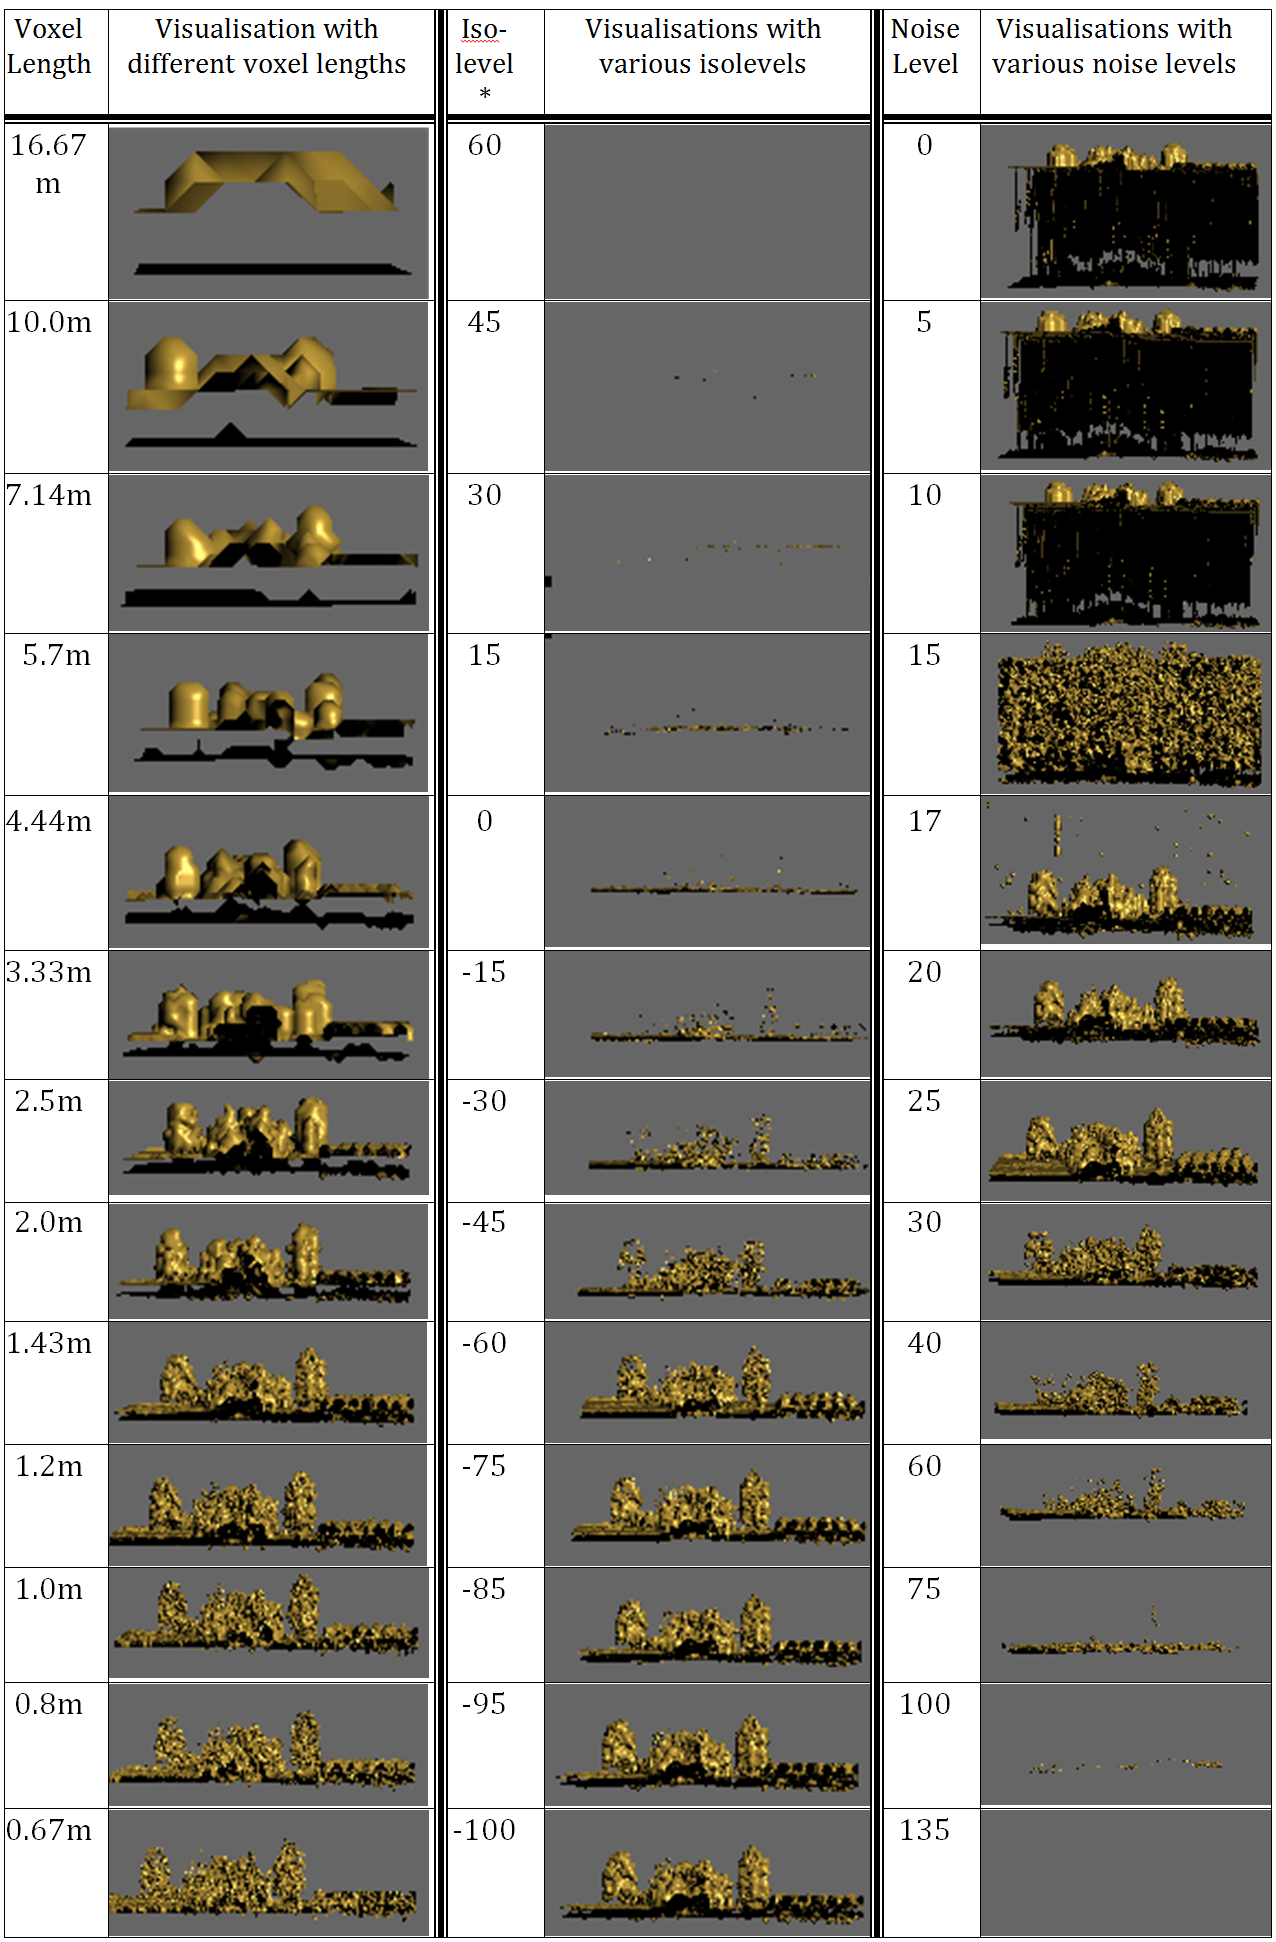
\includegraphics[width=0.95\textwidth]{img/SwitchingParameters}
  	\caption[Polygonisation Parameters]{How the output polygon mesh is affected by modifying the user-defined parameters}
  	\label{fig:SwitchingVisParameters}
  \end{figure}
  
   \begin{figure} [h!]
	   	\centering
    	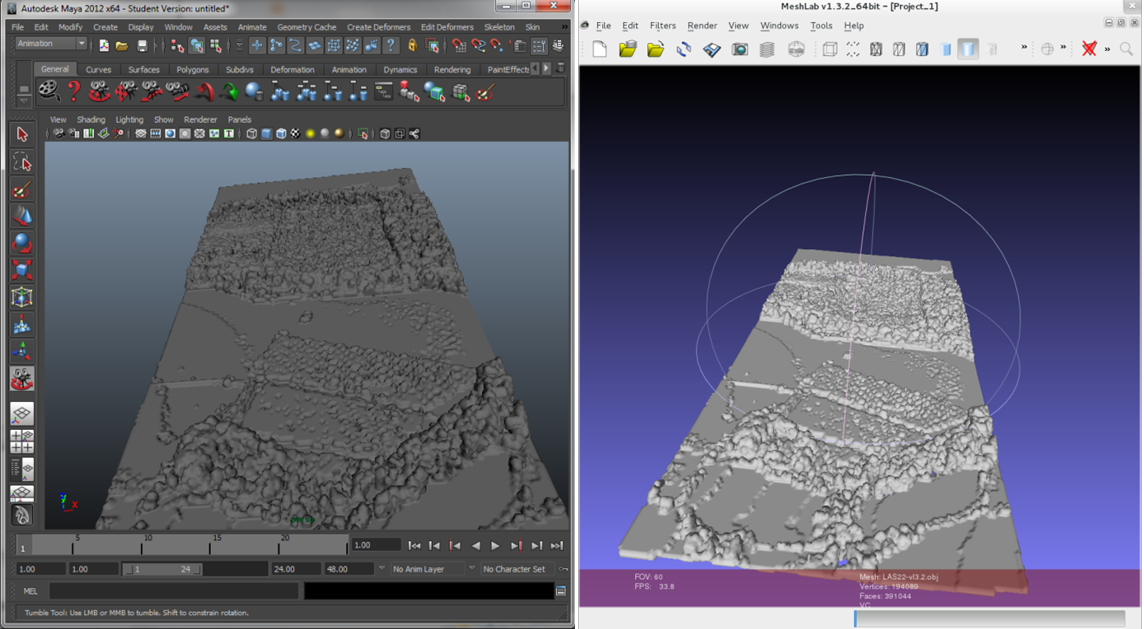
\includegraphics[width=0.9\textwidth]{img/AimationPackages.png}
     	\caption[Animation Packages]{Visualising the output of DASOS into animation software packages (Maya and Meshlab)}
     	\label{fig:AnimationPackages}
    \end{figure}
  
   \begin{figure} [h!]
   	\centering
   	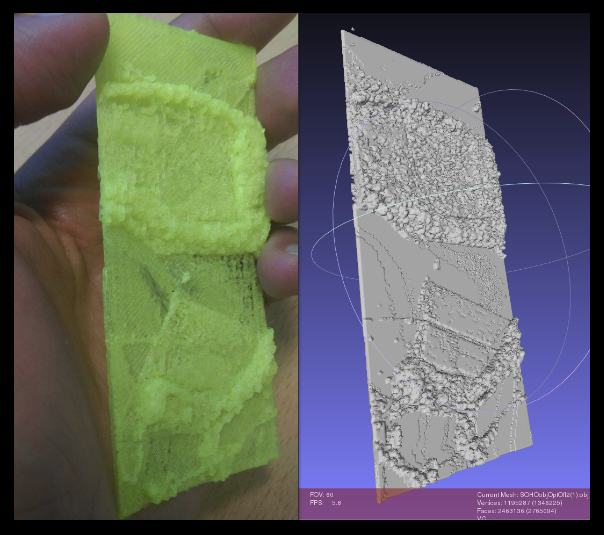
\includegraphics[width=0.9\textwidth]{img/NF-3Dprint}
   	\caption[3D printing]{3D printing of New Forest FW LiDAR data}
   	\label{fig:3Dprinting}
   \end{figure}

 

\end{document}